## Objetivos

\textcolor{blue}{Objetivos generales:}\newline

Al final del curso, los alumnos deberán ser capaces de enfrentar problemas, y como solución diseñar un algoritmo e
implementarlo en un lenguaje de programación.

\vfill
\pause

\vspace{1em}

\textcolor{blue}{Objetivos Específicos:}\newline

\begin{columns}[onlytextwidth,t]
\column{0.7\textwidth}
Los alumnos deberán ser capaces de diseñar algoritmos y programarlos en el lenguaje Python.
\column{0.3\textwidth}

\includegraphics[width=0.9\textwidth,valign=t]{img/xpython_sh-340x340.png}
\end{columns}

\vfill


## Reglas del juego

- La copia en actividades de evaluación se sanciona con nota 1.0, tanto para el que copia como para quien se deja copiar.
- Los controles se realizarán en horario de ayudantía.
- La asistencia tanto a cátedra como a las ayudantías es voluntaria. Sin embargo, lo
expuesto en ellas se puede preguntar
eventualmente en los controles.
- El comportamiento en clases debe ser acorde.


## Recomendaciones

\vfill

- Hacer las guías de ejercicios que se les entreguen.
    - De manera individual, o en grupos de dos personas.
- Leer e investigar para profundizar.
- Resolver nuevos problemas o variantes.
- Consultar inmediatamente al profesor cuando tengan dudas.
- Aprovechar las ayudantías.

\vfill

## Algoritmos

- ¿Qué es un algoritmo?

\pause

- Bueno, según la ``RAE'':

\begin{block}{Algoritmo}

    \justifying
 \begin{small}
 Quizá del lat. tardío *algobarismus, y este abrev. del árabe clásico hisabu lgubar ``cálculo mediante cifras arábigas''.\\[1em]
 \end{small}

 \alert<3->{1. m. Conjunto ordenado y finito de operaciones que permite hallar la solución de un problema.\\[1em]}

 2. m. Método y notación en las distintas formas del cálculo.

\end{block}


## Algoritmos

\bgncolumns

\column{0.6\textwidth}

\vspace{-1em}

- ¿A quién le debemos este concepto?

\pause

\bgnblockgood[wd=.8\textwidth]
Abu Abdallah Muhammad ibn Musa al-Jhwarizmi 
\trmblockgood

\column{0.4\textwidth}
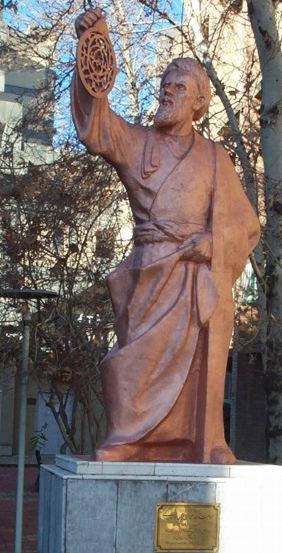
\includegraphics[width=0.4\textwidth,valign=t]{img/Khwarizmi_Amirkabir_University_of_Technology.png}
\trmcolumns

\pause

- Persa del siglo IX (vivió entre el 780 y el 850 aprox.).
- Introdujo el concepto matemático de algoritmo
- Matemático, astrónomo y geógrafo. 
- Padre del álgebra e introductor de nuestro sistema de numeración.
- No es mucho lo que se sabe de su vida.

## Algoritmos

\bgncolumns
\column{0.6\textwidth}
\vspace{-1em}

- ¡¡Esperen!!
- Hay alguien más...

\pause

\bgnblockgood[wd=.8\textwidth]
Euclides
\trmblockgood

\column{0.4\textwidth}
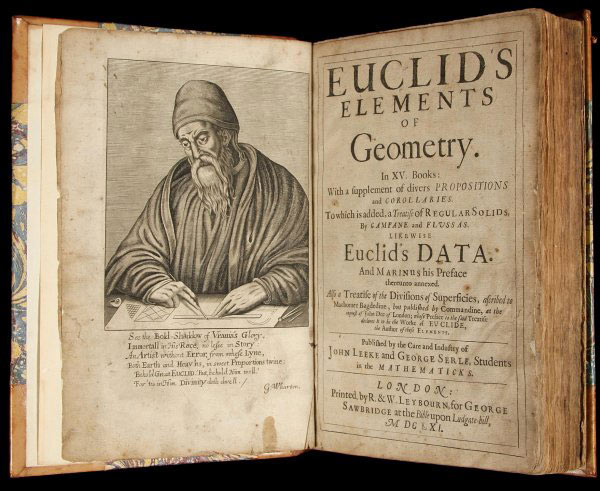
\includegraphics[width=0.9\textwidth,valign=t]{img/euclid-elements.jpg}
\trmcolumns

\pause

- Matemático griego, del siglo IV AC (vivió entre el 325 AC y el 265 AC aprox.).
- Es el padre de la geometría.
- Entre otras muchas cosas nos legó:
    - Un método para encontrar el máximo común divisor de dos números.
    - Este método, por su estructura, también se considera un antecedente de la \textit{algoritmia}.


## Cómo resolver un problema

\vspace{1em}
\begin{small}
\begin{tikzpicture}[node distance=2cm]
  \node (a1) [simplestep] {Identificar el problema};
  \node (a2) [simplestep, opacity=\opacityblock, right=10mm of a1] {Diseñar un algoritmo};
  \node (a3) [simplestep, opacity=\opacityblock, right=10mm of a2] {Programar la solución};
  \draw [arrow] (a1) -- (a2);
  \draw [arrow] (a2) -- (a3);
\end{tikzpicture}
\end{small}

\vfill

- \textbf{Identificar el problema}, ser capaces de describirlo con la menor cantidad de palabras posible.
- Identificar los \textbf{parámetros de entrada} del problema:
    - Los datos necesarios para que nuestro algoritmo funcione.
- Determinar cuáles son las \textbf{salidas} y \textbf{mensajes} esperados al
resolver un problema.


## Cómo resolver un problema

\vspace{1em}
\begin{small}
\begin{tikzpicture}[node distance=2cm]
  \node (a1) [simplestep, opacity=\opacityblock] {Identificar el problema};
  \node (a2) [simplestep, right=10mm of a1] {Diseñar un algoritmo};
  \node (a3) [simplestep, opacity=\opacityblock, right=10mm of a2] {Programar la solución};
  \draw [arrow] (a1) -- (a2);
  \draw [arrow] (a2) -- (a3);
\end{tikzpicture}
\end{small}

\vfill

- \textbf{Identificar los pasos} necesarios para resolver el problema.
- Reconocer las \textbf{condiciones aplicables} para lograr
resolver un problema.
    - Determinar dónde y cómo varían estas condiciones a medida que se avanza en la resolución de un problema.
- \textbf{Diagramar} estos pasos, para hacerse una idea gráfica de la solución.

## Cómo resolver un problema

\vspace{1em}
\begin{small}
\begin{tikzpicture}[node distance=2cm]
  \node (a1) [simplestep, opacity=\opacityblock] {Identificar el problema};
  \node (a2) [simplestep, opacity=\opacityblock, right=10mm of a1] {Diseñar un algoritmo};
  \node (a3) [simplestep, right=10mm of a2] {Programar la solución};
  \draw [arrow] (a1) -- (a2);
  \draw [arrow] (a2) -- (a3);
\end{tikzpicture}
\end{small}

\vfill

- \textbf{Codificar} el programa final en algún lenguaje de programación.
- Una buen algoritmo, no debiera depender del lenguaje que se use finalmente.


## Algoritmos: entrada y salida

\simpleTitle[0mm]{Respecto de la Entrada y Salida debemos tener claro que:}

- Un algoritmo es un \strongText{sistema}, compuesto de diversos elementos, que se \strongText{comunica} con el exterior \strongText{recibiendo} y \strongText{entregando} datos.
- Es muy importante definir \strongText{qué} se recibe y \strongText{cuándo}.
- Análogamente hay que definir \strongText{qué} se entrega y \strongText{cuándo}.

\vfill

\begin{center}
\begin{tikzpicture}[font=\sffamily\small,baseline={($(current bounding box.center)+(0,-0.5ex)$)},
        ->,
        >=stealth',
        thick,
    ]
    \node at (-4,1.5) (e1) {Entrada};
    \node at (-3.5,0.5) (e2) {Entrada};
    \node at (-5,-0.25) (e4) {Entrada};
    \node at (-4.5,-1) (e3) {Entrada};
    \node at (3.5,1.5) (s1) {Mensaje};
    \node at (4.5,0) (s2) {Salida};
    \node at (4,-1) (s3) {Mensaje};
    \node[ellipse, draw, fill=red!30, minimum height=20mm, minimum width=40mm] at (0,0) (sist) {Algoritmo};
    \draw (e1) edge[out=20,in=100] (sist);
    \draw (e2) edge[out=10,in=140] (sist);
    \draw (e3) edge[out=-20,in=-120] (sist);
    \draw (e4) edge[out=-20,in=190] (sist);
    \draw (sist) edge[out=50,in=180] (s1);
    \draw (sist) edge[out=0,in=180] (s2);
    \draw (sist) edge[out=-20,in=180] (s3);
\end{tikzpicture}
\end{center}

## Algoritmos: entrada y salida
\simpleTitle{¿Cómo identificarlas?}

- Analicemos varios ejemplos:

    1. Calcular el área de un círculo.
    
        \begin{itemize}
            \item <2-> \textcolor{blue}{Entrada: radio.}
            \item <2-> \textcolor{blue}{Salida: área calculada.}
        \end{itemize}
    1. Calcular el área de un rectángulo.
        \begin{itemize}
            \item <3-> \textcolor{blue}{Entrada: largo de los dos lados.}
            \item <3-> \textcolor{blue}{Salida: área calculada.}
        \end{itemize}
    1. Cargar la BIP (desde el punto de vista del cajero).
        \begin{itemize}
            \item <4-> \textcolor{blue}{Entrada: tarjeta, monto a cargar y dinero entregado.}
            \item <4-> \textcolor{blue}{Salida: tarjeta ya cargada y vuelto.}
        \end{itemize}

## Un ejemplo de la vida cotidiana

\simpleTitle{Supongamos que queremos comprar paltas:}

- Tenemos un presupuesto fijo para ello.
    - Por ejemplo, no compraremos más caro que \$2.500 por kilo, y debemos comprar dos kilos.
- En nuestro vecindario hay un determinado número de verdulerías.
    - Por ejemplo, hay cuatro verdulerías de confianza en el barrio.

\pause

\bgnblocknormal[wd=.9\textwidth,centered=true]
\textbf{Objetivo:}\newline Identificar las entradas y salidas en este problema.
\trmblocknormal
